
%% bare_conf.tex
%% V1.4
%% 2012/12/27
%% by Michael Shell
%% See:
%% http://www.michaelshell.org/
%% for current contact information.
%%
%% This is a skeleton file demonstrating the use of IEEEtran.cls
%% (requires IEEEtran.cls version 1.8 or later) with an IEEE conference paper.
%%
%% Support sites:
%% http://www.michaelshell.org/tex/ieeetran/
%% http://www.ctan.org/tex-archive/macros/latex/contrib/IEEEtran/
%% and
%% http://www.ieee.org/

%%*************************************************************************
%% Legal Notice:
%% This code is offered as-is without any warranty either expressed or
%% implied; without even the implied warranty of MERCHANTABILITY or
%% FITNESS FOR A PARTICULAR PURPOSE! 
%% User assumes all risk.
%% In no event shall IEEE or any contributor to this code be liable for
%% any damages or losses, including, but not limited to, incidental,
%% consequential, or any other damages, resulting from the use or misuse
%% of any information contained here.
%%
%% All comments are the opinions of their respective authors and are not
%% necessarily endorsed by the IEEE.
%%
%% This work is distributed under the LaTeX Project Public License (LPPL)
%% ( http://www.latex-project.org/ ) version 1.3, and may be freely used,
%% distributed and modified. A copy of the LPPL, version 1.3, is included
%% in the base LaTeX documentation of all distributions of LaTeX released
%% 2003/12/01 or later.
%% Retain all contribution notices and credits.
%% ** Modified files should be clearly indicated as such, including  **
%% ** renaming them and changing author support contact information. **
%%
%% File list of work: IEEEtran.cls, IEEEtran_HOWTO.pdf, bare_adv.tex,
%%                    bare_conf.tex, bare_jrnl.tex, bare_jrnl_compsoc.tex,
%%                    bare_jrnl_transmag.tex
%%*************************************************************************

% *** Authors should verify (and, if needed, correct) their LaTeX system  ***
% *** with the testflow diagnostic prior to trusting their LaTeX platform ***
% *** with production work. IEEE's font choices can trigger bugs that do  ***
% *** not appear when using other class files.                            ***
% The testflow support page is at:
% http://www.michaelshell.org/tex/testflow/



% Note that the a4paper option is mainly intended so that authors in
% countries using A4 can easily print to A4 and see how their papers will
% look in print - the typesetting of the document will not typically be
% affected with changes in paper size (but the bottom and side margins will).
% Use the testflow package mentioned above to verify correct handling of
% both paper sizes by the user's LaTeX system.
%
% Also note that the "draftcls" or "draftclsnofoot", not "draft", option
% should be used if it is desired that the figures are to be displayed in
% draft mode.
%
\documentclass[conference]{IEEEtran}
% Add the compsoc option for Computer Society conferences.
%
% If IEEEtran.cls has not been installed into the LaTeX system files,
% manually specify the path to it like:
% \documentclass[conference]{../sty/IEEEtran}
\usepackage{comment}
\usepackage{hyperref}




% Some very useful LaTeX packages include:
% (uncomment the ones you want to load)


% *** MISC UTILITY PACKAGES ***
%
%\usepackage{ifpdf}
% Heiko Oberdiek's ifpdf.sty is very useful if you need conditional
% compilation based on whether the output is pdf or dvi.
% usage:
% \ifpdf
%   % pdf code
% \else
%   % dvi code
% \fi
% The latest version of ifpdf.sty can be obtained from:
% http://www.ctan.org/tex-archive/macros/latex/contrib/oberdiek/
% Also, note that IEEEtran.cls V1.7 and later provides a builtin
% \ifCLASSINFOpdf conditional that works the same way.
% When switching from latex to pdflatex and vice-versa, the compiler may
% have to be run twice to clear warning/error messages.






% *** CITATION PACKAGES ***
%
%\usepackage{cite}
% cite.sty was written by Donald Arseneau
% V1.6 and later of IEEEtran pre-defines the format of the cite.sty package
% \cite{} output to follow that of IEEE. Loading the cite package will
% result in citation numbers being automatically sorted and properly
% "compressed/ranged". e.g., [1], [9], [2], [7], [5], [6] without using
% cite.sty will become [1], [2], [5]--[7], [9] using cite.sty. cite.sty's
% \cite will automatically add leading space, if needed. Use cite.sty's
% noadjust option (cite.sty V3.8 and later) if you want to turn this off
% such as if a citation ever needs to be enclosed in parenthesis.
% cite.sty is already installed on most LaTeX systems. Be sure and use
% version 4.0 (2003-05-27) and later if using hyperref.sty. cite.sty does
% not currently provide for hyperlinked citations.
% The latest version can be obtained at:
% http://www.ctan.org/tex-archive/macros/latex/contrib/cite/
% The documentation is contained in the cite.sty file itself.






% *** GRAPHICS RELATED PACKAGES ***
%
\ifCLASSINFOpdf
  \usepackage[pdftex]{graphicx}
  % declare the path(s) where your graphic files are
  % \graphicspath{{../pdf/}{../jpeg/}}
  % and their extensions so you won't have to specify these with
  % every instance of \includegraphics
  % \DeclareGraphicsExtensions{.pdf,.jpeg,.png}
\else
  % or other class option (dvipsone, dvipdf, if not using dvips). graphicx
  % will default to the driver specified in the system graphics.cfg if no
  % driver is specified.
  \usepackage[dvips]{graphicx}
  % declare the path(s) where your graphic files are
  % \graphicspath{{../eps/}}
  % and their extensions so you won't have to specify these with
  % every instance of \includegraphics
  % \DeclareGraphicsExtensions{.eps}
\fi
% graphicx was written by David Carlisle and Sebastian Rahtz. It is
% required if you want graphics, photos, etc. graphicx.sty is already
% installed on most LaTeX systems. The latest version and documentation
% can be obtained at: 
% http://www.ctan.org/tex-archive/macros/latex/required/graphics/
% Another good source of documentation is "Using Imported Graphics in
% LaTeX2e" by Keith Reckdahl which can be found at:
% http://www.ctan.org/tex-archive/info/epslatex/
%
% latex, and pdflatex in dvi mode, support graphics in encapsulated
% postscript (.eps) format. pdflatex in pdf mode supports graphics
% in .pdf, .jpeg, .png and .mps (metapost) formats. Users should ensure
% that all non-photo figures use a vector format (.eps, .pdf, .mps) and
% not a bitmapped formats (.jpeg, .png). IEEE frowns on bitmapped formats
% which can result in "jaggedy"/blurry rendering of lines and letters as
% well as large increases in file sizes.
%
% You can find documentation about the pdfTeX application at:
% http://www.tug.org/applications/pdftex





% *** MATH PACKAGES ***
%
%\usepackage[cmex10]{amsmath}
% A popular package from the American Mathematical Society that provides
% many useful and powerful commands for dealing with mathematics. If using
% it, be sure to load this package with the cmex10 option to ensure that
% only type 1 fonts will utilized at all point sizes. Without this option,
% it is possible that some math symbols, particularly those within
% footnotes, will be rendered in bitmap form which will result in a
% document that can not be IEEE Xplore compliant!
%
% Also, note that the amsmath package sets \interdisplaylinepenalty to 10000
% thus preventing page breaks from occurring within multiline equations. Use:
%\interdisplaylinepenalty=2500
% after loading amsmath to restore such page breaks as IEEEtran.cls normally
% does. amsmath.sty is already installed on most LaTeX systems. The latest
% version and documentation can be obtained at:
% http://www.ctan.org/tex-archive/macros/latex/required/amslatex/math/





% *** SPECIALIZED LIST PACKAGES ***
%
%\usepackage{algorithmic}
% algorithmic.sty was written by Peter Williams and Rogerio Brito.
% This package provides an algorithmic environment fo describing algorithms.
% You can use the algorithmic environment in-text or within a figure
% environment to provide for a floating algorithm. Do NOT use the algorithm
% floating environment provided by algorithm.sty (by the same authors) or
% algorithm2e.sty (by Christophe Fiorio) as IEEE does not use dedicated
% algorithm float types and packages that provide these will not provide
% correct IEEE style captions. The latest version and documentation of
% algorithmic.sty can be obtained at:
% http://www.ctan.org/tex-archive/macros/latex/contrib/algorithms/
% There is also a support site at:
% http://algorithms.berlios.de/index.html
% Also of interest may be the (relatively newer and more customizable)
% algorithmicx.sty package by Szasz Janos:
% http://www.ctan.org/tex-archive/macros/latex/contrib/algorithmicx/




% *** ALIGNMENT PACKAGES ***
%
%\usepackage{array}
% Frank Mittelbach's and David Carlisle's array.sty patches and improves
% the standard LaTeX2e array and tabular environments to provide better
% appearance and additional user controls. As the default LaTeX2e table
% generation code is lacking to the point of almost being broken with
% respect to the quality of the end results, all users are strongly
% advised to use an enhanced (at the very least that provided by array.sty)
% set of table tools. array.sty is already installed on most systems. The
% latest version and documentation can be obtained at:
% http://www.ctan.org/tex-archive/macros/latex/required/tools/


% IEEEtran contains the IEEEeqnarray family of commands that can be used to
% generate multiline equations as well as matrices, tables, etc., of high
% quality.




% *** SUBFIGURE PACKAGES ***
%\ifCLASSOPTIONcompsoc
%  \usepackage[caption=false,font=normalsize,labelfont=sf,textfont=sf]{subfig}
%\else
%  \usepackage[caption=false,font=footnotesize]{subfig}
%\fi
% subfig.sty, written by Steven Douglas Cochran, is the modern replacement
% for subfigure.sty, the latter of which is no longer maintained and is
% incompatible with some LaTeX packages including fixltx2e. However,
% subfig.sty requires and automatically loads Axel Sommerfeldt's caption.sty
% which will override IEEEtran.cls' handling of captions and this will result
% in non-IEEE style figure/table captions. To prevent this problem, be sure
% and invoke subfig.sty's "caption=false" package option (available since
% subfig.sty version 1.3, 2005/06/28) as this is will preserve IEEEtran.cls
% handling of captions.
% Note that the Computer Society format requires a larger sans serif font
% than the serif footnote size font used in traditional IEEE formatting
% and thus the need to invoke different subfig.sty package options depending
% on whether compsoc mode has been enabled.
%
% The latest version and documentation of subfig.sty can be obtained at:
% http://www.ctan.org/tex-archive/macros/latex/contrib/subfig/




% *** FLOAT PACKAGES ***
%
%\usepackage{fixltx2e}
% fixltx2e, the successor to the earlier fix2col.sty, was written by
% Frank Mittelbach and David Carlisle. This package corrects a few problems
% in the LaTeX2e kernel, the most notable of which is that in current
% LaTeX2e releases, the ordering of single and double column floats is not
% guaranteed to be preserved. Thus, an unpatched LaTeX2e can allow a
% single column figure to be placed prior to an earlier double column
% figure. The latest version and documentation can be found at:
% http://www.ctan.org/tex-archive/macros/latex/base/


%\usepackage{stfloats}
% stfloats.sty was written by Sigitas Tolusis. This package gives LaTeX2e
% the ability to do double column floats at the bottom of the page as well
% as the top. (e.g., "\begin{figure*}[!b]" is not normally possible in
% LaTeX2e). It also provides a command:
%\fnbelowfloat
% to enable the placement of footnotes below bottom floats (the standard
% LaTeX2e kernel puts them above bottom floats). This is an invasive package
% which rewrites many portions of the LaTeX2e float routines. It may not work
% with other packages that modify the LaTeX2e float routines. The latest
% version and documentation can be obtained at:
% http://www.ctan.org/tex-archive/macros/latex/contrib/sttools/
% Do not use the stfloats baselinefloat ability as IEEE does not allow
% \baselineskip to stretch. Authors submitting work to the IEEE should note
% that IEEE rarely uses double column equations and that authors should try
% to avoid such use. Do not be tempted to use the cuted.sty or midfloat.sty
% packages (also by Sigitas Tolusis) as IEEE does not format its papers in
% such ways.
% Do not attempt to use stfloats with fixltx2e as they are incompatible.
% Instead, use Morten Hogholm'a dblfloatfix which combines the features
% of both fixltx2e and stfloats:
%
% \usepackage{dblfloatfix}
% The latest version can be found at:
% http://www.ctan.org/tex-archive/macros/latex/contrib/dblfloatfix/




% *** PDF, URL AND HYPERLINK PACKAGES ***
%
%\usepackage{url}
% url.sty was written by Donald Arseneau. It provides better support for
% handling and breaking URLs. url.sty is already installed on most LaTeX
% systems. The latest version and documentation can be obtained at:
% http://www.ctan.org/tex-archive/macros/latex/contrib/url/
% Basically, \url{my_url_here}.




% *** Do not adjust lengths that control margins, column widths, etc. ***
% *** Do not use packages that alter fonts (such as pslatex).         ***
% There should be no need to do such things with IEEEtran.cls V1.6 and later.
% (Unless specifically asked to do so by the journal or conference you plan
% to submit to, of course. )


% correct bad hyphenation here
\hyphenation{op-tical net-works semi-conduc-tor}


\begin{document}
%
% paper title
% can use linebreaks \\ within to get better formatting as desired
% Do not put math or special symbols in the title.
\title{A Review of Caching Techniques for Low Power Consumption in Embedded Devices}

% author names and affiliations
% use a multiple column layout for up to three different
% affiliations
\author{\IEEEauthorblockN{Aniket Ashwin Samant}
\IEEEauthorblockA{Delft University of Technology\\
Delft, The Netherlands\\
Email: A.A.Samant@student.tudelft.nl}
\and
\IEEEauthorblockN{Apoorva Arora}
\IEEEauthorblockA{Delft University of Technology\\
Delft, The Netherlands\\
Email: A.Arora-1@student.tudelft.nl}
\and
\IEEEauthorblockN{Snehal Jauhri}
\IEEEauthorblockA{Delft University of Technology\\
Delft, The Netherlands\\
Email: S.Jauhri@student.tudelft.nl}
}
% conference papers do not typically use \thanks and this command
% is locked out in conference mode. If really needed, such as for
% the acknowledgment of grants, issue a \IEEEoverridecommandlockouts
% after \documentclass

% for over three affiliations, or if they all won't fit within the width
% of the page, use this alternative format:
% 
%\author{\IEEEauthorblockN{Michael Shell\IEEEauthorrefmark{1},
%Homer Simpson\IEEEauthorrefmark{2},
%James Kirk\IEEEauthorrefmark{3}, 
%Montgomery Scott\IEEEauthorrefmark{3} and
%Eldon Tyrell\IEEEauthorrefmark{4}}
%\IEEEauthorblockA{\IEEEauthorrefmark{1}School of Electrical and Computer Engineering\\
%Georgia Institute of Technology,
%Atlanta, Georgia 30332--0250\\ Email: see http://www.michaelshell.org/contact.html}
%\IEEEauthorblockA{\IEEEauthorrefmark{2}Twentieth Century Fox, Springfield, USA\\
%Email: homer@thesimpsons.com}
%\IEEEauthorblockA{\IEEEauthorrefmark{3}Starfleet Academy, San Francisco, California 96678-2391\\
%Telephone: (800) 555--1212, Fax: (888) 555--1212}
%\IEEEauthorblockA{\IEEEauthorrefmark{4}Tyrell Inc., 123 Replicant Street, Los Angeles, California 90210--4321}




% use for special paper notices
%\IEEEspecialpapernotice{(Invited Paper)}




% make the title area
\maketitle

% As a general rule, do not put math, special symbols or citations
% in the abstract
\begin{abstract}
Embedded systems that operate in the low-power domain need to be as efficient as possible in terms of their components' power consumption, including the on-board processors'. Caches in processors, specifically instruction caches, are known to be power-hungry since instructions are fetched frequently for the processor's operations. This paper reviews and compares some caching techniques specifically intended to lower the power consumption of the instruction cache. The ideas of tiny caches, filter caches and Reduced One-Bit Tag Instruction Cache are discussed and qualitatively compared. These techniques are also compared with traditional instruction caches in terms of performance degradation (if any) and power savings achieved during normal operation.    
\newline \newline
\textit{\textbf{Keywords: caching, dynamic power,  embedded systems, filter cache, instruction cache, loop cache, low power, short backward branch, tag}}
\end{abstract}


\IEEEpeerreviewmaketitle


\section{Introduction}
Most of the dynamic power consumed by an embedded processor is through instruction-fetching \cite{segars}. The reason is that it occurs in most cycles, involves switching of large numbers of high capacitance wires, and makes accesses to set-associative caches - all of this collectively consumes a lot of power \cite{1}. Thus, it also lays the foundation for using caching techniques in embedded processors to minimize power consumption while fetching instructions.

\begin{comment}
One such technique is to use a very small instruction cache (64 to 512 bytes in size) called a \textit{tiny cache}. Accessing tiny caches consumes less power because of very short wires inside the cache, and also because these caches can be integrated close to the microprocessor resulting in shorter and less power-consuming bus lines.\cite{1} 
\end{comment}

%\section{ Introduce the topic and its relevance to computer architecture.}
There are two main research facets of this paper:
\begin{itemize}
    \item \textit{Fundamental ideas behind the introduced caching techniques and their operation} 
    \item \textit{Factors which influence the power savings for a particular caching technique}
\end{itemize}

In this paper, we first review multiple tiny cache designs - starting with a direct-mapped filter cache, and then followed by loop caches: dynamic, pre-loaded and hybrid loop caches. All the discussed tiny cache designs are then compared for their power reduction, main instruction-memory access reduction and overall impact on performance. We also discuss and review the energy savings for a cache design that employs a small cache size and a one-bit tag comparison. This kind of cache, the Reduced One-Bit Tag Instruction Cache (ROBTIC), is also aimed at achieving significant power reductions. \textit{This review paper specifically focuses on the findings from \cite{1,fc1,robtic}.}

We see that the techniques explained in this paper indeed reduce the power consumed by the cache subject to certain limitations, as will be explored in the forthcoming sections. We also note that filter caches in general are more suited for applications involving larger instruction block sizes whereas loop caches and ROBTIC are better suited for applications with tiny instruction blocks; however, customization of the caches can be performed as per prior information about the applications.

\begin{comment}
\textit{\textbf{Main Conclusions of the Investigation}}
\begin{itemize}
    \item Direct mapped tiny filter cache reduces instruction fetch power by 50\% but incurs significant performance overhead
    \item Loop caches are tagless and hit is always guaranteed hence they eliminate performance overheads 
    \item Dynamically loaded loop caches reduces fetches to regular instruction memory by about 30\% and preloaded loop caches achieve about a 60\% reduction
       \item One-level hybrid dynamic/preloaded loop cache work best on average in terms of energy savings.
    \item Loop caches can thus be used as an energy saving methodology in embedded processors.
     \item ROBTIC is a design proposed for the Level 1 cache, unlike other discussed tiny cache designs which are in Level 0 of the memory hierarchy. This design of I-cache is shown to reduce power consumption by upto 48\% and also reduces the area overhead.
\end{itemize}
\end{comment}

In the first section, we evaluate the design technique of the filter cache. Loop caches are discussed next (dynamically loaded, pre-loaded, and one- and two-level hybrid loop caches) and compared with traditional I-caches. The ROBTIC is introduced and discussed in the following section, after which some comparisons are drawn between the introduced techniques. The paper ends with some conclusions and ideas for selecting an optimal cache design.

\section{Evaluated caching techniques}

In this section, we first discuss \textit{filter cache} and explain the concept behind it. We follow it up with a discussion on \textit{loop caching} techniques and the advantages they can offer over filter caches. We cover the dynamically loaded tag-less loop caching technique, pre-loaded loop caches and then introduce hybrid loop caching. We conclude the section with \textit{ROBTIC}, a different approach aimed at reducing tag comparisons without much additional overhead.

\subsection{Filter Cache}

	A Filter Cache (FC) can offer substantial energy savings in embedded low power applications. The authors of \cite{fc1} discuss the concept behind using a filter cache and its advantages. Moreover, a method of designing a filter cache whose size is tuned to an application is described. This method uses loop profiling of the application to determine a filter cache size that would maximize savings by reducing the number of accesses to the main Instruction Cache.
	
	\subsubsection{Concept}
	Filter Cache (FC) is a small, direct mapped intermediate cache that sits between the processor and the first instruction cache (or L1 cache). It is typically of much smaller size than the L1 cache and its objective is to reduce the number of accesses to the L1 cache. It does this by storing the next instructions for all the small loops of the program. This avoids unnecessary accesses to the L1 cache. In this way, since the larger L1 cache is not cycled, it leads to substantial energy savings.
	
	\subsubsection{Points of consideration}
	Due to its small size and placement close to the execution core, Filter Caches can lead to substantial energy savings, especially if a majority of loops in an application can be serviced using it. Since the loop characteristics of an application can be easily obtained, the Filter Cache can be designed specific to the application. Optimal design of the FC has shown energy reduction numbers above 50\% for certain applications~\cite{fc2}.
	
	However, a point to consider when adding a FC is that when a cache access 'miss' takes place in the FC (when the required next instruction is not present in the Filter cache), then the L1 cache has to be accessed. Since we now need an extra step to fetch from the L1 cache (going through the Filter Cache), this leads to an overhead and reduces the performance.
	
	To avoid this performance reduction, a parallel prediction method is described in \cite{fc1}. This method uses an extra parallel path to access the L1 (main) cache. Moreover, a predictor is used which can predict whether the next instruction can be fetched from the FC or not. If the next instruction cannot be fetched from the FC, the alternate parallel path is used to directly access the L1 cache. This avoids the extra step through the FC in case of a miss and leads to a performance improvement (See Figure 1). Modern predictors can achieve close to 90\% accuracy in prediction and a design for them is mentioned in~\cite{fc3}.

\begin{figure}[!h]
	\centering
	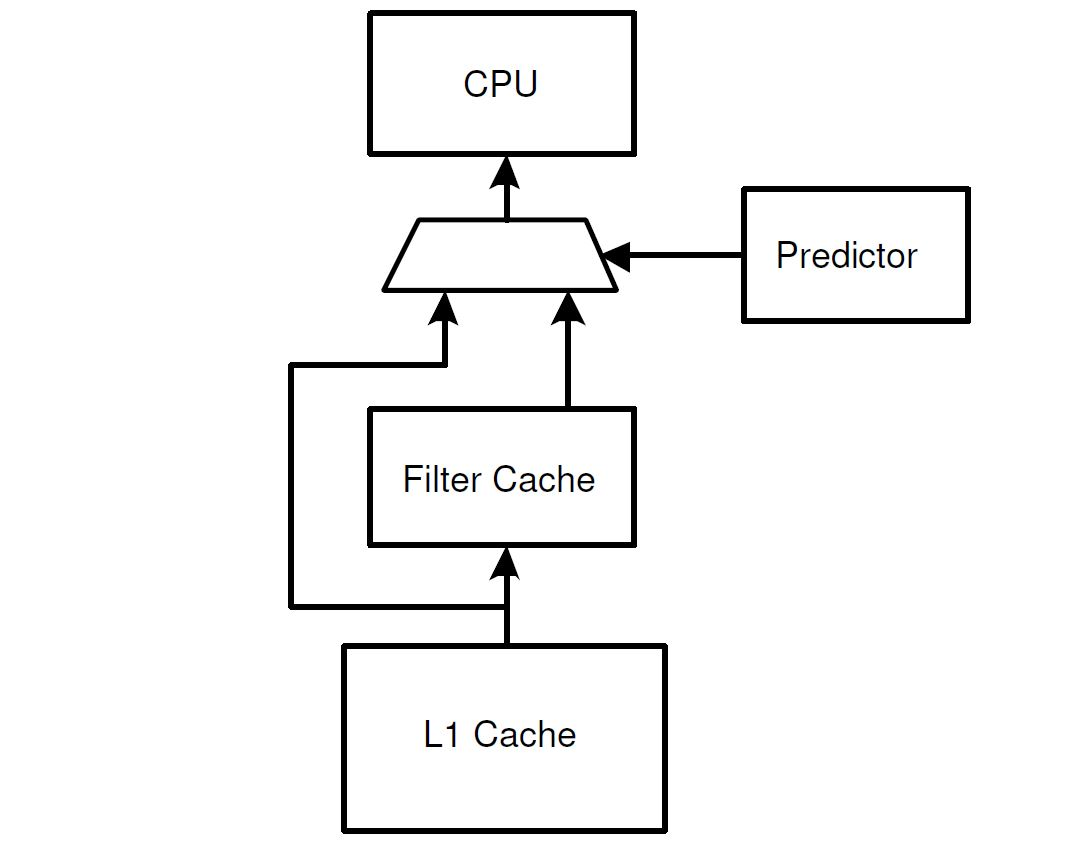
\includegraphics[width=2.5in]{images/PredictiveFilterCache.JPG}
	\caption{A Predictive Filter Cache \cite{fc1}}
	\label{Predictive Filter Cache}
\end{figure}
	
	\subsubsection{Choosing FC size using Loop Profiling}
	Designing of the FC for an application implies choosing a FC size that can accommodate a majority of the loops in the application to achieve maximum hits and hence maximize power saving. Note that the FC size cannot be too big otherwise it ends up consuming too much power by itself (due to accesses and static power consumption of such a large cache). A design methodology is described in \cite{fc1} that uses loop profiling to analyze the application and accordingly chooses a FC size. To avoid unnecessarily long computations, FC size is chosen from a fixed set of: 128, 256, 512 bytes etc.
	
	Given a binary file of the application, Loop profiling is done using algorithms that generate a Control Flow Graph of the program and analyze the back edges of the graph to identify loops. Note that within a loop, the part of the code within it which is executed in at least 20\% of the loop's iterations is chosen to be cached in the FC. Once the loops are identified, the energy savings for these loops are calculated analytically and the size with the best relative energy saving is chosen.
	\begin{itemize}
    \item\textbf{Energy savings}: Usage of a 256 byte filter cache results in a power reduction of 58\% with a 21\% performance reduction \cite{fc2}. Moreover, a comparison was made using eighteen applications from MediaBench between choosing an optimal size for the FC for an application as compared to using a 256 byte FC for all the applications. Tuning the FC using the mentioned design strategy and finding optimal size was found to, on average, further lead to 11\% energy savings as compared to general usage of a FC of 256 bytes for all the applications \cite{fc1}.

\end{itemize}
	
\subsection{Loop Caching Techniques}

As discussed above, similar to the mechanism in a traditional cache, a direct-mapped filter cache also stores part of the address of each instruction, and compares the tag with the desired address to determine a cache hit or miss. Whenever a miss occurs, a microprocessor stall occurs. Tag accesses and comparisons require some energy overhead, while stalls due to misses cause performance and energy overhead \cite{1}. To eliminate these overheads, loop caching techniques were introduced as discussed below:\\

\subsubsection{Dynamically Loaded Loop Cache}

\begin{itemize}
    \item A dynamic loop cache is a tiny cache which is free from tags and misses unlike a filter cache. Whenever a loop is detected in the dynamic instruction flow through a short backwards branch (sbb) instruction, the cache controller is triggered to fill the tiny cache in the next iteration of this small loop. This fill is non-intrusive and the processor continues to fetch and execute from main instruction memory. When the sbb is detected again, the instruction fetch is switched to the loop cache. The fetch continues from this loop cache until the loop is exited \cite{1}.
    \item The advantage of using a dynamic loop cache over a filter cache is that, firstly, no tag comparisons are required in the loop cache, thus reducing overhead and power per access. Secondly, performance does not degrade since filling is done non-intrusively and a hit is always guaranteed which avoids any CPU stalls \cite{1}.
    \item\textbf{Energy Savings}: Running Powerstone and MediaBench benchmarks on MIPS and Superscalar respectively, the energy savings results using dynamic loop cache were obtained and examined. It was observed that on average energy savings for all benchmarks was 22\% \cite{1}. The experiments with dynamic loop caching show that minimizing the power within the loop cache itself is not a high priority, which makes sense as this power is very small compared to L1 fetching. To really improve a loop cache, the number of supported loops needs to be increased. This is the motivation behind a Pre-loaded Loop cache design.
\end{itemize}
\subsubsection{Pre-loaded Loop Cache}

\begin{itemize}
    \item In a pre-loaded loop cache, the the entire loop is stored in the loop cache
during the  the microprocessor boot sequence, before the program begins executing. First, the program is profiled to detect critical loops. These are the most frequently executed loops which are stored in the loop cache. Unlike the dynamic loop cache, a pre-loaded loop cache can support change of flow instructions and subroutines and stores multiple loops and subroutines simultaneously \cite{1}.
 \begin{figure}[!h]
	\centering
	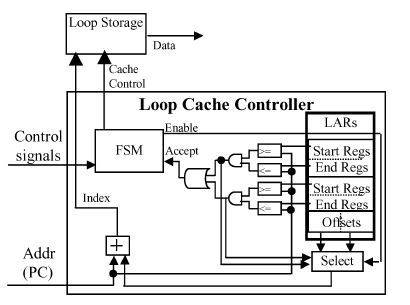
\includegraphics[width=2.9in]{images/fig4.JPG}
	\caption{Architecture of a pre-loaded loop cache \cite{1}.}
	\label{}
\end{figure}
\item As shown in Figure 2, a pre-loaded loop cache consists of loop storage, a loop cache controller, and loop address registers (LARs) \cite{1}. The loop cache controller is responsible for filling the loop cache, switching instruction fetches from main instruction memory to the loop cache and vice-versa.
    \item \textbf{Energy Savings}: Improvement in the loop cache hit rates for both MediaBench on SimpleScalar and Powerstone on MIPS was reported. This justifies the observed improvement in the average instruction fetch energy savings of 66\% \cite{1}.
    \begin{figure}[!h]
	\centering
	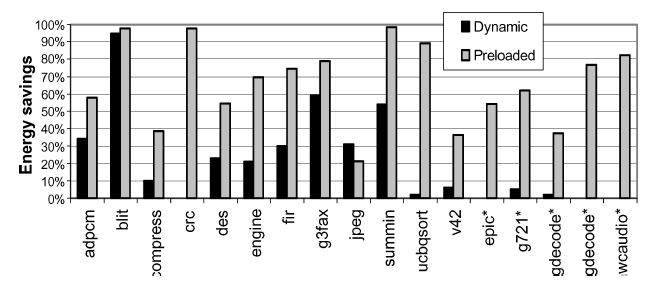
\includegraphics[width=3.5 in]{images/fig7.JPG}
	\caption{Percentage of instruction fetch energy saved by dynamic and pre-loaded caches using a 128-instruction loop cache \cite{1}.}
	\label{}
\end{figure}
\end{itemize}

\subsubsection{Hybrid Pre-loaded/Dynamic Loop Cache }
It was reported that for some benchmarks dynamic loop cache performed better while for some pre-loaded performed better \cite{1}. This became the motivation for designing a hybrid cache which behaved like both dynamic and pre-loaded loop cache.\newline
\textit{One Level Hybrid}\newline
In the one-level hybrid loop cache, part of the cache storage holds pre-loaded loops, while the rest of the storage is filled dynamically. Thus, the pre-loaded part does not store loops that are handled by dynamic loop caching.\newline
\textit{Two Level Hybrid}\newline
In a two level hybrid cache, a second level of the storage holds pre-loaded loops while the first level of storage acts like a dynamic loop cache. Moreover, when a short backwards branch is detected, the first (dynamic) level could be filled in both from regular memory or from the second level (pre-loaded) storage. If a change of flow occurs, the target address is checked against the loop address registers. If a match occurs, then the first level loop storage is filled with the appropriate loop from the second level.
\begin{itemize}
    \item\textbf{Energy savings}: Simulation results showed that the one-level hybrid loop cache reduces main instruction memory fetching by 50\% for both benchmark suites, even with a very small cache size of 32 instructions with a dynamic portion of 16 instructions \cite{1}. On the other hand, the two level
scheme does not seem to perform as well as the other loop caching methods. \cite{1}
\end{itemize}

\subsection{The ROBTIC}

The previously described caching techniques involve the addition of a tiny cache block next to the L1 cache. However, it is also possible to optimize the L1 cache block itself, without the addition of a separate cache block; that is the fundamental idea behind this caching technique. In a traditional instruction cache, the tag accounts for a considerable proportion of the chip area and also consumes a lot of power (for example, a 20-bit tag mapped to a 32-bit PC address leads to the tag occupying about 37.7\% of the cache area, in addition to a 20-bit comparator circuitry \cite{robtic}). To reduce the area occupied by the tag and consequently the tag-comparator size, J.Gu et al \cite{robtic} introduce a new cache design, namely the ROBTIC, or the Reduced One-Bit Tag Instruction Cache, which employs a technique involving a comparison of just one bit (the LSB) of the tag \cite{robtic}. There is some additional circuitry involved, but the overall power consumption is lower compared with a traditional cache's case.

ROBTIC's scheme takes advantage of the spatial and temporal locality of programs for which its usage is intended, so as to achieve low power consumption without compromising on the performance of the cache. The main point to note is that in ROBTIC, there is no extra cache block involved as is the case with loop caches, filter caches etc; cache tag comparison reduction is the main idea.

\subsubsection{High-level architecture}

\begin{figure}[!h]
	\centering
	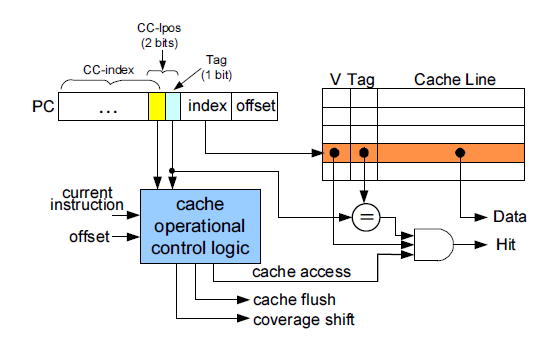
\includegraphics[width=3.2in]{images/architecture_ROBTIC.PNG}
	\caption{ROBTIC Architecture \cite{robtic}}
	\label{fig:robtic_arch}
\end{figure}

A ROBTIC cache is similar to a traditional cache in terms of its structure - for every cache entry there is a valid bit, a tag field, and a \textit{cache line (for data)} - however, the tag field is only one bit wide. The valid bit together with the tag bit is used to determine a cache hit or miss. This modification does require some additional circuitry though, and it is present in the form of a cache operational control unit, which will be explained in a more detailed fashion soon. But as Figure \ref{fig:robtic_arch} suggests, the overall architecture is quite similar to a traditional cache's.

\subsubsection{Assumptions made}

There are some assumptions made regarding the ROBTIC cache's operation, viz.:
\begin{itemize}
	\item The applications that run on the processor mainly involve \textit{loop basic blocks}, that is, instruction blocks that are repeatedly fetched and hence are spatially and temporally local. 
	\item A cache line holds multiple instructions, all instructions being of equal size 
	\item A standard cache size of 32 lines ($2^5$) is defined for ROBTIC, based on surveys suggesting that more than 90\% of loops contain fewer than 30 instructions \cite{survey1} \cite{survey2}
	\item The instruction cache is directly mapped to avoid the cache replacement policy issue (that is, if there are sets present in the cache, an algorithm would be needed to decide which exact cache items must be replaced).
\end{itemize}

\subsubsection{ROBTIC Operation}

The authors of \cite{robtic} define cache coverage (CC) as the "cache-mappable address space" of the main memory. In a full-tag cache, the tag size is chosen so as to map the entire memory address space using the cache tag; that is, to have the entire memory space in the CC. However, in ROBTIC, since the tag size is one bit, the tag by itself cannot be used for covering the entire address space. 

Thus, for CC in ROBTIC, the first few MSBs from the program counter (PC) are used directly along with the 1-bit tag to uniquely determine a cache block; the first few MSBs, collectively constituting the "MSB set", form the \textit{CC-index} as shown in Figure \ref{fig:robtic_arch}. 
\textit{We clearly see that we are left with only a 1-bit comparison and a series of small operations for determining the CC-index, instead of a full-tag comparison, which is a much more power-hungry operation. This is how the ROBTIC achieves its power consumption reduction.}
\\
The CC-index changes when the PC changes its MSB set based on the instruction block to be executed. The existing cache is flushed and the next set of instructions gets cached (corresponding to the next CC-index).

\subsubsection{A point to consider} In an ideal case, all instructions in a block would be aligned so as to be local to a CC-indexed block.
However, generally, a block of instructions could also be spread over two CC-index values (that is, the instruction block could have parts in different CC-index values) and cause an undesired cycle of cache flushing brought about by the two parts of the instruction block evicting each other for every execution cycle (referred to as the "Ping-pong effect" in \cite{robtic}). To tackle this issue, an "overlapped dynamic cache coverage control" scheme is proposed.

\subsubsection{Dynamic cache coverage scheme}
The main focus is on not flushing the cache immediately when the CC-index changes, and letting the currently cached instructions finish execution instead. The authors discuss three control flows that could arise in the ROBTIC's operation states, viz.:
\begin{itemize}
	\item Cache coverage shift (CCS): When the CC-index changes due to the PC's movement, the cache may need to be retained or flushed depending on how the loop block is positioned in memory.
	\item Cache flush: Invalidates all the instruction entries in the cache. It is assumed that all jump instructions and branch instructions with an offset larger than the cache size should be followed by a cache flush operation (hops are assumed to be long distance in such cases.)
	\item Normal Cache Access: As is the case with a traditional cache, if a PC address is within the current CC region and the instruction to be executed gets a hit in the cache, it should be fetched and executed normally.
\end{itemize}

\subsubsection{Algorithm for detecting CCS}
A crude and straightforward method of detecting "\textit{overlapped cache coverage}" is to compare the top and bottom tags of the CC region with the PC address's full tag to know if a CCS is involved, and take actions accordingly. However, with the full-tag comparison involved, the purpose of having a 1-bit tag is defeated.
Hence, the authors of \cite{robtic} make use of a simpler approach in which only three consecutive CC regions need to be differentiated to determine if a CCS occurs, and this differentiation is performed on the basis of the two LSBs of the full tag from the PC (referred to as the "\textit{CC-lpos}", as shown in Figure \ref{fig:robtic_arch}). The CC-lpos bits are converted to their corresponding Gray code representation and it is used to determine if a CCS takes place. Two values need to be stored - the "common value" (\textbf{CV}) of the Gray code representation (i.e. the bit value between consecutive 2-bit Gray-code numbers that doesn't change), and its corresponding bit position (\textbf{CVP}). The Gray code representation of the CC-lpos for each new PC address is computed, and the common value is checked with the CC region's common value. If they're the same, a normal cache access is performed, and if different, it implies the CC region needs to be shifted. The new CC region's CV and CVP values are calculated accordingly.
This algorithm clearly requires very little additional circuitry and hence does not significantly increase the chip area or the power consumption.

\begin{itemize}
\item \textbf{Energy Savings:} The ROBTIC cache design was tested by the authors of \cite{robtic} on applications from the Motorola Powerstone and MiBench benchmark suites and compared with the results obtained by running the same applications on a traditional cache design. For a general ROBTIC cache (with 32 cache lines) power savings and performance metrics were compared, and in most cases the ROBTIC cache provided a significant amount of power savings (in the range of 25 to 30\%) at almost the same performance; the authors noted a few cases, however, in which there was a significant performance degradation due to non-locality of programs. Furthermore, for specific applications in which the loop block size is considerably different, varying the size of the ROBTIC cache between 8 and 128 lines added to the overall power savings due to the increased cache hit rate.
\end{itemize}

\section{Comparative Study: Caching Techniques}
This paper reviews various caching techniques for low power consumption as explained in the above sections in detail. In this section we highlight some of the advantages and disadvantages of each of discussed techniques to aid a comparative study.
\newline
\newline
\textit{\textbf{Filter vs. Loop Caches}}\\
On reviewing the papers on Filter and Loop caching techniques, we see that for a small loop cache of size 32 instructions, a one-level hybrid loop cache gives maximum energy savings \cite{1}. On the other hand for larger sizes of the caches, a filter cache performs the best (Filter cache achieves more than 50\% energy savings for Powerstone benchmarks \cite{fc1}).

Figure 5 highlights the difference in memory hierarchy of the filter and loop cache.
A key advantage of loop caches is that they are tag-less and thus hits are guaranteed, resulting in no performance overhead. When this relative performance overhead is large enough, it also leads to less energy consumption as compared to the filter cache.

\begin{figure}[!h]
	\centering
	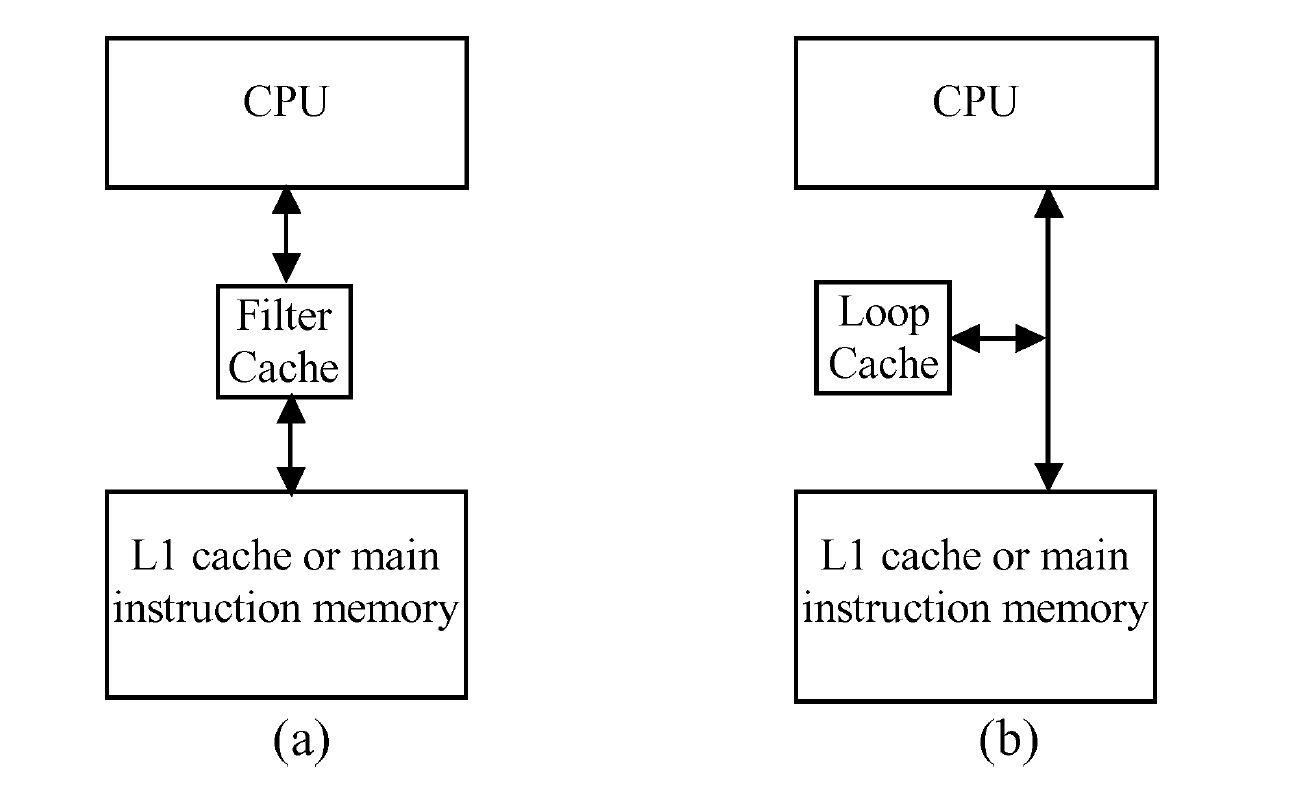
\includegraphics[width=2.8in]{images/compare1.JPG}
	\caption{Memory hierarchy roles for (a) a filter cache (b) a loop cache \cite{1}.}
	\label{Comparison_Cache}
\end{figure}

\begin{table}
\centering
	\caption{A comparison of Loop Caching techniques}
	\label{table:loop_cache}
	\begin{tabular}{ | p{1.5cm} | p{1.3cm} |p{2.5cm} |}
			\hline
		\textbf{Type of Loop Cache} & \textbf{Average Energy Savings}	&  	\textbf{L1 cache access reduction}  \\ \hline
			Dynamic & 30\%  & 30\% L1 fetch reduction no matter how large the loop cache size \\ \hline
		Preloaded Loop cache &	 66\%  &40\% for
a loop cache of size 32 instructions with six preloaded regions of code. \\ \hline
		One Level Hybrid &	60\%  & 50\% for
a loop cache of size 32 instructions and dynamic portion of 16 instructions		\\ \hline
Two-Level Hybrid & 56\% & 30\% for
first level size of 32 instructions 		\\ \hline
		\end{tabular}
		\smallskip
		
		\textit{(Energy savings are for a 128-Instruction Dynamic Loop Cache for Powerstone benchmarks \cite{1})}
		
	\end{table}
A comparison of the different loop caching techniques was done in \cite{1} and is summarized in Table \ref{table:loop_cache}. We can conclude from this comparison that among the loop caching methods, the one-level hybrid loop cache seems the better choice. It achieves more energy savings than a pure dynamic loop cache. Though the one-level hybrid performs slightly worse than a pre-loaded loop cache, it also has the advantage of operating in a dynamic-only mode and avoid pre-loading altogether and hence is a better choice.\newline\\
\textit{\textbf{Comparing ROBTIC with Filter and Loop Caches}} \newline
Filter and loop caches are supplementary caches added to an existing L1 cache to reduce main memory accesses and hence have to be small enough so as to not offset the benefit of reduced access times with the demerit of increased area. The ROBTIC, on the other hand, is a scheme for reduced tag comparisons in the instruction cache, since the tag comparison circuitry otherwise accounts for significant power consumption. Unlike the filter cache and the loop cache, ROBTIC is a kind of I-cache with a different scheme for fetching cached data, rather than a supplementary cache to an existing I-cache. Given that the complexity of the logic involved is constant, this scheme is scalable to larger sizes of the cache and memory, so as to get reduced area and energy consumption with little or no performance loss.

There are some limitations to the ROBTIC cache though: jump instructions needn't always lead to a cache flush, and could be handled based on whether the jump is long or within the CC area. Moreover, ROBTIC is only a direct-mapped cache without any associativity (as stated in the initial assumptions).
	

\section{Conclusions}

Each of the evaluated caching techniques relies heavily on its target applications being \textit{local} (that is, having successive instruction addresses close to each other), Since this is the case in most embedded applications \cite{robtic}; they are all viable solutions for low power consumption in embedded applications with lots of loop-basic blocks. Moreover, given the fact that most embedded processors run the same application throughout their lifetime of operation, the caching technique and the cache size can be customized as per the application. Thus, we can choose between the evaluated caching solutions based on the application's loop profile and the area available for a supplementary cache (For filter and loop caches).

We can conclude that:
\begin{itemize}
    \item A Filter Cache offers size-able power savings provided it can service most of the loops in an application while still remaining relatively small in size as compared to the L1 cache. A majority of the performance degradation due to the filter cache can be mitigated by using an accurate parallel predictive path which directly accesses the L1 cache when needed \cite{fc3}.
    \item In the case where the application constitutes of tiny loops or the area available for a supplementary cache is small, loop caches become more favourable (can be made as small as just 32 instructions\cite{1}). This is because there are no tag comparisons and a hit is guaranteed in a loop cache. Hence, tiny loops can be directly serviced without CPU stalls or performance degradation, unlike in a filter cache.
    \item Between different loop caching methods, a one-level hybrid solution seems most favourable due to relatively larger power savings from the tests in \cite{1}; as well as the fact that it can both be pre-loaded with loop instructions and dynamically service tiny loops.
    \item In the case where adding a supplementary cache is undesired, the ROBTIC design approach can be considered. For an application with many loop basic blocks, it offers virtually no performance degradation but significant power savings. Moreover, the area added is small since it is limited to the control blocks needed to implement this solution. However, a major drawback to this approach is the fact that it is only for direct-mapped caches. This significantly reduces the scope for this solution. %and thus is only viable for systems with a direct mapped L1 cache or willingness to shift to a direct-mapped cache which significantly reduces the scope for this solution.
\end{itemize}
(A relative comparison of caching techniques is shown in Table II.)

	\begin{table}[t]
	\centering
		\caption{Relative comparison of the presented caching techniques}
		\begin{tabular}{ | p{1.7cm} | p{1.7cm} |p{1.7cm} | p{1.7cm} |}
			\hline
			Parameters	& \textbf{Filter cache} &  	\textbf{Loop cache} &	\textbf{ROBTIC}\\ \hline
			\textbf{Area increase} &	Yes &	Yes	& Minimal \\ \hline
			\textbf{Target program assumptions} & Lots of loop basic blocks present	& Tiny loop basic blocks present	&	Lots of loop basic blocks present\\ \hline
			\textbf{Relative Power savings} & Large & Large for small cache sizes & Limited \\ \hline
			\textbf{Cache type} & Direct-mapped	& Tag-less	&	Direct-mapped \\ \hline
			\textbf{Performance degradation}	& Large if no parallel prediction	& Minimal & Minimal\\ \hline
			\textbf{L1 cache access reduction}	& Large	& Large if program has mostly tiny loops	&N/A (ROBTIC is the L1 cache)\\ \hline
		\end{tabular}
		\label{table:caching_comp}
	\end{table}
\begin{comment}
\textbf{Look at the research questions : both should be entertained here! Also put one line in abstract!!}
Summarise the report content and draw the conclusions of your investigation.
%"Start with filter cache."
%Filter cache, the most effective in energy reduction,
%has been shown to achieve 58\% power saving at the cost
%of 21\% performance loss. Adding predictive [15, 16, 14] \cite{2}
%capability to the filter cache hierarchy reduces the performance
%penalty associated with the hierarchical access of the
%filter cache.
"However,,,,, filter cache has 21\% performance loss."
% The paper mentions a technique to quickly find an optimum filter cache size. However, even optimised for size, there are these drawbacks.
We can see from the described caching techniques that there is no clear \textit{winner} in terms of reducing area and achieving 
\end{comment}	
\begin{comment}
\begin{appendices}

\section{Some Observations}

\begin{itemize}
\item  Do not use titles like "Reading Assignment Report - Group x". Give the report a meaningful title such that the reader can infer form it the essence of the discussed topic. 
\item Plagiarism rules are still in place despite the fact that the introduction of novel ideas is not the key issue. Do not make use of text from the papers under discussions or any other papers, reports, etc.
\item More references can and should be included, if relevant, in the text.
\end{itemize}

\end{appendices}
\end{comment}
% An example of a floating figure using the graphicx package.
% Note that \label must occur AFTER (or within) \caption.
% For figures, \caption should occur after the \includegraphics.
% Note that IEEEtran v1.7 and later has special internal code that
% is designed to preserve the operation of \label within \caption
% even when the captionsoff option is in effect. However, because
% of issues like this, it may be the safest practice to put all your
% \label just after \caption rather than within \caption{}.
%
% Reminder: the "draftcls" or "draftclsnofoot", not "draft", class
% option should be used if it is desired that the figures are to be
% displayed while in draft mode.
%
%\begin{figure}[!t]
%\centering
%\includegraphics[width=2.5in]{myfigure}
% where an .eps filename suffix will be assumed under latex, 
% and a .pdf suffix will be assumed for pdflatex; or what has been declared
% via \DeclareGraphicsExtensions.
%\caption{Simulation Results.}
%\label{fig_sim}
%\end{figure}

% Note that IEEE typically puts floats only at the top, even when this
% results in a large percentage of a column being occupied by floats.


% An example of a double column floating figure using two subfigures.
% (The subfig.sty package must be loaded for this to work.)
% The subfigure \label commands are set within each subfloat command,
% and the \label for the overall figure must come after \caption.
% \hfil is used as a separator to get equal spacing.
% Watch out that the combined width of all the subfigures on a 
% line do not exceed the text width or a line break will occur.
%
%\begin{figure*}[!t]
%\centering
%\subfloat[Case I]{\includegraphics[width=2.5in]{box}%
%\label{fig_first_case}}
%\hfil
%\subfloat[Case II]{\includegraphics[width=2.5in]{box}%
%\label{fig_second_case}}
%\caption{Simulation results.}
%\label{fig_sim}
%\end{figure*}
%
% Note that often IEEE papers with subfigures do not employ subfigure
% captions (using the optional argument to \subfloat[]), but instead will
% reference/describe all of them (a), (b), etc., within the main caption.


% An example of a floating table. Note that, for IEEE style tables, the 
% \caption command should come BEFORE the table. Table text will default to
% \footnotesize as IEEE normally uses this smaller font for tables.
% The \label must come after \caption as always.
%
%\begin{table}[!t]
%% increase table row spacing, adjust to taste
%\renewcommand{\arraystretch}{1.3}
% if using array.sty, it might be a good idea to tweak the value of
% \extrarowheight as needed to properly center the text within the cells
%\caption{An Example of a Table}
%\label{table_example}
%\centering
%% Some packages, such as MDW tools, offer better commands for making tables
%% than the plain LaTeX2e tabular which is used here.
%\begin{tabular}{|c||c|}
%\hline
%One & Two\\
%\hline
%Three & Four\\
%\hline
%\end{tabular}
%\end{table}


% Note that IEEE does not put floats in the very first column - or typically
% anywhere on the first page for that matter. Also, in-text middle ("here")
% positioning is not used. Most IEEE journals/conferences use top floats
% exclusively. Note that, LaTeX2e, unlike IEEE journals/conferences, places
% footnotes above bottom floats. This can be corrected via the \fnbelowfloat
% command of the stfloats package.






% conference papers do not normally have an appendix


% use section* for acknowledgement
%\section*{Acknowledgment}
%
%
%The authors would like to thank...
%




% trigger a \newpage just before the given reference
% number - used to balance the columns on the last page
% adjust value as needed - may need to be readjusted if
% the document is modified later
%\IEEEtriggeratref{8}
% The "triggered" command can be changed if desired:
%\IEEEtriggercmd{\enlargethispage{-5in}}

% references section

% can use a bibliography generated by BibTeX as a .bbl file
% BibTeX documentation can be easily obtained at:
% http://www.ctan.org/tex-archive/biblio/bibtex/contrib/doc/
% The IEEEtran BibTeX style support page is at:
% http://www.michaelshell.org/tex/ieeetran/bibtex/
%\bibliographystyle{IEEEtran}
% argument is your BibTeX string definitions and bibliography database(s)
%\bibliography{IEEEabrv,../bib/paper}
%
% <OR> manually copy in the resultant .bbl file
% set second argument of \begin to the number of references
% (used to reserve space for the reference number labels box)
\begin{thebibliography}{5}
\bibitem{segars}
Segars, S.\emph{Low power design techniques for microprocessors}, IEEE International Solid-State Circuits Conference, 2001. 
\bibitem{1}
Ann Gordon-Ross, Susan Cotterell and Frank Vahid, \emph{Tiny Instruction Caches For Low Power Embedded Systems}, ACM Transactions on Embedded Computing Systems, Vol. 2, No. 4, November 2003, Pages 449–481.
\bibitem{fc1}
K. Vivekanandarajah and T. Srikanthan, \emph{Custom instruction filter cache synthesis for low-power embedded systems}, 16th IEEE International Workshop on Rapid System Prototyping (RSP'05), Montreal, Que., 2005, pp. 151-157.
\bibitem{robtic}
J. Gu and H. Guo and P. Li, \emph{ROBTIC: An On-chip Instruction Cache Design for Low Power Embedded Systems}, 2009 15th IEEE International Conference on Embedded and Real-Time Computing Systems and Applications.
\bibitem{fc2}
Kin J. Gupta M. and Mangione-Smith W.H.  \emph{Filtering memory references to increase energy efficiency}, Computers IEEE Transactions on Volume: 49 Issue: 1 pp. 1-15 Jan 2000.
\bibitem{fc3}
K. Vivekanandarajah T. Srikanthan and S. Bhattacharyya \emph{Energy-delay efficient filter cache hierarchy using pattern prediction scheme}, IEE Proceedings - Computers and Digital Techniques Vol. 151.Issue 2 March 2004.
\bibitem{survey1}
C.-L. Yang and C.-H. Lee, \emph{Hotspot cache: Joint temporal and spatial
locality exploitation for icache energy reduction}, Proceedings of
ISLPED’04, 2004, pp. 114–119.
\bibitem{survey2}
K. Ali, M. Aboelaze, and S. Datta, \emph{Reducing energy in instruction caches
by using multiple line buffers with prediction}, Lecture Notes in Computer
Science, v 4759 LNCS., pp. 508–521, 2008.
\end{thebibliography}




% that's all folks
\end{document}

